\begin{figure}[htbp]
\centering
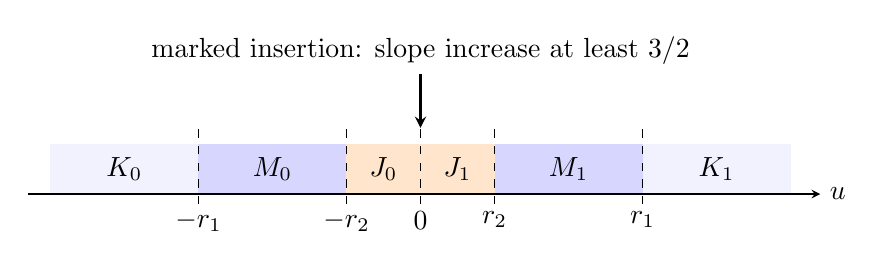
\begin{tikzpicture}[x=.94cm,y=.8cm,>=stealth]
 \fill[blue!5] (-5,0) rectangle (-3,.8);
 \fill[blue!16] (-3,0) rectangle (-1,.8);
 \fill[orange!20] (-1,0) rectangle (1,.8);
 \fill[blue!16] (1,0) rectangle (3,.8);
 \fill[blue!5] (3,0) rectangle (5,.8);
 \draw[->] (-5.3,0)--(5.4,0) node[right] {$u$};
 \foreach \x in {-3,-1,0,1,3} {\draw[dashed] (\x,-.16)--(\x,1.05);}
 \node at (-4,.4) {$K_0$};
 \node at (-2,.4) {$M_0$};
 \node at (-.5,.4) {$J_0$};
 \node at (.5,.4) {$J_1$};
 \node at (2,.4) {$M_1$};
 \node at (4,.4) {$K_1$};
 \node[below] at (-3,-.12) {$-r_1$};
 \node[below] at (-1,-.12) {$-r_2$};
 \node[below] at (0,-.12) {$0$};
 \node[below] at (1,-.12) {$r_2$};
 \node[below] at (3,-.12) {$r_1$};
 \draw[->,thick] (0,1.9)--(0,1.05);
 \node[above,align=center] at (0,1.9) {marked insertion: slope increase at least $3/2$};
\end{tikzpicture}
\caption{The two radial scales, with $r_i=6\log a_i$ and $a_1\ge a_2$.
The central region suppresses both sets of strict roots and is compared
with $J_t$. The next region suppresses only the first set and is compared
with $M_t$; the exterior is compared with $K_t$. The transitions have
width $O(\delta\log k)$ in the proof. The diagram is schematic and does
not depict the exceptional case in which the middle intervals disappear.}
\label{fig:radial-regions}
\end{figure}
